\chapter{ArrowPipe: An arrow interface for writing SPar expressions}
When trying to express more complicated and interesting parallel patterns, e.g map or reduce, We realize SPar is too low-level so that it is difficult to express simple computation because of overheads of expressing communication patterns by hand. In addition, compilation from Par-Alg to SPar is hard since they are very different domain specific languages. 

To solve both issues, we draw inspirations from the Arrow interface (in particular, work done by \cite{braunArrowsParallelComputation2018} where they use arrow interface to express parallel computation) and introduce ArrowPipe.

ArrowPipe is an arrow interface for writing SPar expressions. Withe the help from ArrowPipe, Users can use canonical arrow combinators to write algorithms in Arrow without writing any explicit communication and gain parallelized algorithms for free. Similarly, ArrowPipe makes hassle-free compilation from Par-Alg to SPar possible because Par-Alg Proto is also an arrow expression and simply interpreting arrow combinators by the ArrowPipe implementations fills the gap between Par-Alg and SPar. 

\section{Syntax}
\begin{listing}[ht]
\inputminted{Haskell}{arrow/def.hs}
\caption{Definition of ArrowPipe}
\label{arrowPipe:def}
\end{listing}
The simplified syntax of ArrowPipe can be found in \coref{arrowPipe:def}. ArrowPipe is a type synonym of \hask{Nat -> Pipe a b}. It consumes \hask{Nat} which means the identifier of a process and output \hask{Pipe a b}. The reson why we use \hask{Nat} as the only parameter is to ensuring no duplication of processes name since in most of the time, duplication is bad for parallelization. It will be explained more thoroughly in \secref{arrowPipe:roleAllc}.

\hask{Pipe a b} data structures is the essential component of ArrowPipe. It regards computation as a pipe where data with type \hask{a} goes into the pipe and data with type \hask{b} get out of the pipe. Internally, it's a record type of four fields. \hask{start} field identifies the process where the input data is received. \hask{cont} field has the type \hask{a -> Proc} which is a continuation waiting for the input data produced by the last pipe. \hask{env} represents a group of Procs interacting inside the pipe to produce the output data, in other words, it is the parallel computation. \hask{end} indicates the process that produces the output data in the end. We can retrieve the corresponding process by a look up on the env with the key \hask{end}. The returned Proc returns a data with type \hask{b}.
\subsection{Arrow interface}
\hask{ArrowPipe} is an instance of Arrow typeclass as well as ArrowChoice type class. For example, the type signature of the combinators \hask{>>>}, \hask{|||}, \hask{&&&} and \hask{arr} are shown below. The main difference between their type signatures and the usual arrow interface is that in the \hask{arr}, the function is wrapped with Core. In general, it captures the same meaning as the usual arrow interfaces. Implementation details of these combinators will be explained in \secref{arrowPipe:impl}.
\begin{code}
\begin{minted}{Haskell}
(>>>) :: (ArrowPipe a b) -> (ArrowPipe b c) -> (ArrowPipe a c)
-- (>>>) :: a b c -> a c d -> a b d
arr :: (Core (a -> b)) -> ArrowPipe a b
-- arr :: (b -> c) -> a b c
(|||) :: (ArrowPipe a c) -> (ArrowPipe b c) -> ArrowPipe (Either a b) c
-- (|||) :: a b d -> a c d -> a (Either b c) d
(&&&) :: (ArrowPipe b c) -> (ArrowPipe b c') -> ArrowPipe b (c, c')
-- (&&&) :: a b c -> a b c' -> a b (c,c')
(***) :: (ArrowPipe b c) -> (ArrowPipe b' c') -> ArrowPipe (b, b') (c, c')
-- (***) :: a b c -> a b' c' -> a (b, b') (c, c')
\end{minted}
\end{code}
\subsection{Example: Parallel programming patterns}
As an example, we will illustrate some typical computation patterns used in parallel computing.
\begin{figure*}[ht]
    \begin{subfigure}[b]{0.475\textwidth}
      \centering
      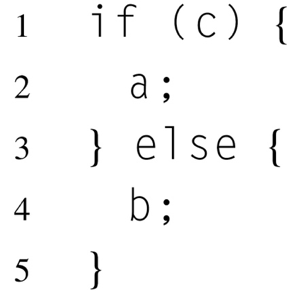
\includegraphics[width=0.7\textwidth]{arrow/code.png}
    \end{subfigure}
    \hfill
    \begin{subfigure}[b]{0.475\textwidth}
      \centering
      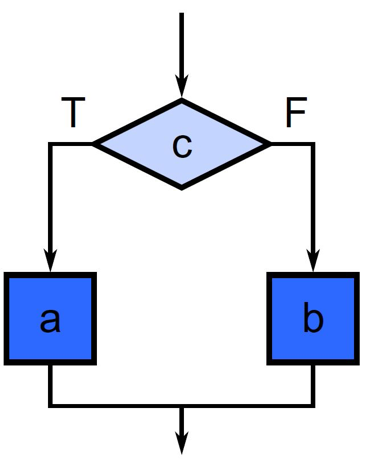
\includegraphics[width=0.7\textwidth]{arrow/select.png}
    \end{subfigure}
    \caption{Visualization of the select pattern \cite{mccoolStructuredParallelPrograming2012}}
    \label{arrowPipe:fig:select}
\end{figure*}

First of all, the select pattern illustrated by \figref{arrowPipe:fig:select} is equivalent to an expression formed by \hask{|||} combinators, where the data constructor \hask{Left} means True and the data constructor \hask{Right} means False for the sum type \hask{Either}.
\begin{figure*}[ht]
    \begin{subfigure}[b]{0.475\textwidth}
       \centering
       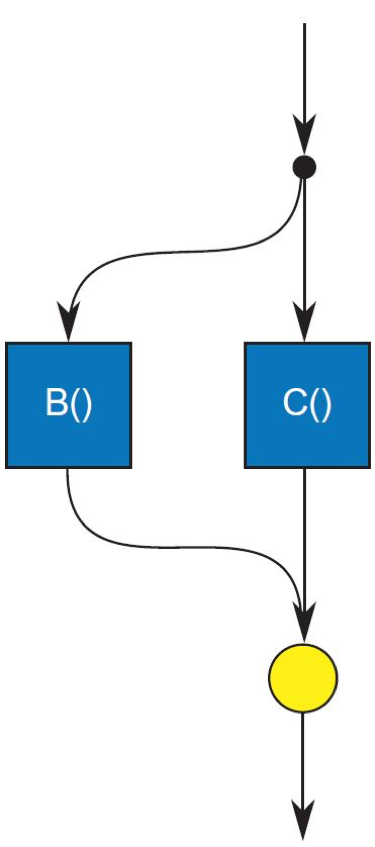
\includegraphics[width=0.60\textwidth]{arrow/fork.png}
        \caption{Visualization of the fork-join pattern \cite{mccoolStructuredParallelPrograming2012}}
        \label{arrowPipe:fig:fork}
    \end{subfigure}
    \hfill
   \begin{subfigure}[b]{0.475\textwidth}
        \centering
        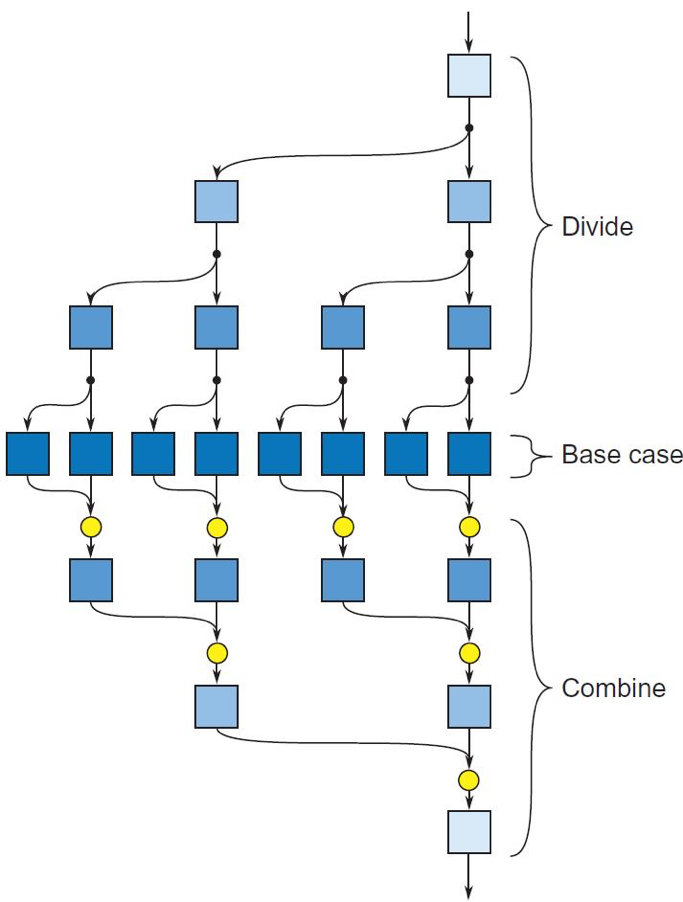
\includegraphics[width=\textwidth]{arrow/dq.png}
        \caption{Fork-Join Pattern for Divide-Conquer \cite{mccoolStructuredParallelPrograming2012}}
        \label{arrowPipe:fig:dq}
    \end{subfigure}
    \caption{Fork-join pattern and divide-and-conquer algorithms}
\end{figure*}
Secondly, the fundamental building block of parallel pattern, the fork-join pattern illustrated by \figref{arrowPipe:fig:fork} can be expressed by \hask{&&&} combinator. The arrowPipe produced by \hask{&&&} has the two-ary tuple as the output type collecting the computation result of the main thread and the forked thread and also acts as a synchronization point.

\begin{listing}[ht]
    \inputminted{Haskell}{arrow/dq.hs}
    \caption{2-ways and 3-levels divided-and-conquer algorithm in arrowPipe}
    \label{arrowPipe:dq}
\end{listing}
In the end, more complicated pattern can be expressed compositely from simpler pattern expressed in ArrowPipe. We can use a typical divide-and-conquer algorithms implemented with fork-join as an example. \figref{arrowPipe:fig:dq} shows a divide-and-conquer algorithms with 2-ways and 3-levels of fork-join. The algorithm can be expressed in arrowPipe shown in \coref{arrowPipe:dq}. The divide-and-conquer pattern can be built recursively in Haskell. For the base case, we simply apply the basic computation. Otherwise, we first call split and then call the function recursively with the level decremented by one and, in the end, call the merge to combine the results. Every expressions in the function definition are connected using arrow combinators. A 3-level divided-and-conquer algorithm is constructed by passing 3 to the function resulting a algorithm with $2^3 = 8$-way parallelism.

The implementation demos the power of implementing ArrowPipe as a domain specific language embedded in Haskell. We make full use of Haskell features, i.e high order functions and polymorphic functions to construct expressive, composable and generic computation patterns.

More examples of algorithms formed by ArrowPipe, e.g. dot product or merge sort are shown in the \secref{eval}.
\section{Implementation of arrow combinators} \label{arrowPipe:impl}
\section{Strategies for optimized role allocation} \label{arrowPipe:roleAllc}
\section{Satisfaction of arrow laws}
% \section{Optimizations}
% \subsection{Fusion}
% \subsection{Upper bound of the number of roles}
% \section{Parallel programming patterns}
% \subsection{Serial control patterns}
% \subsection{Fork-join pattern for Divide and conquer}
% \subsection{Reduce}
\section{Conclusions}
Arrow interface is the perfect interface to express general computation for this project because not only is it intuitive to understand and visualize but also its combinators \hask{***} and \hask{&&&} has built-in parallel natural.

So far, we've used ArrowPipe to help us compile Par-Alg to SPar. The remained challenge is the code generation from SPar to the target platform which will be illustrated in the next chapter.
% \section{Applications}
% \subsection{Hassle-free compilation from ParAlg to ArrowPipe} %Hassle-free
% \subsection{An interface for arrow computation with automatic parallelization}
% \section{Power of arrow and EDSL: expressibility and composability}
% \subsection{Arrow interface}
% \subsection{Haskell as the host language}